%%%%%%%%%%%%%%%%%%%%%%%%%%%%%%%%%%%%%%%%%%%%%%%%%%%%%%%%%%%%%%%%%%%%%%%%%%%%%%%%
%2345678901234567890123456789012345678901234567890123456789012345678901234567890
%        1         2         3         4         5         6         7         8

\documentclass[letterpaper, 10 pt, conference]{ieeeconf}  % Comment this line out if you need a4paper

%\documentclass[a4paper, 10pt, conference]{ieeeconf}      % Use this line for a4 paper

\IEEEoverridecommandlockouts                              % This command is only needed if 
                                                          % you want to use the \thanks command

\overrideIEEEmargins                                      % Needed to meet printer requirements.

% See the \addtolength command later in the file to balance the column lengths
% on the last page of the document

% The following packages can be found on http:\\www.ctan.org
%\usepackage{graphics} % for pdf, bitmapped graphics files
%\usepackage{epsfig} % for postscript graphics files
%\usepackage{mathptmx} % assumes new font selection scheme installed
%\usepackage{times} % assumes new font selection scheme installed
%\usepackage{amsmath} % assumes amsmath package installed
%\usepackage{amssymb}  % assumes amsmath package installed



\usepackage{amsmath,amssymb}
\usepackage{tikz,hyperref,graphicx,units,subfig}
\usepackage{sidecap,wrapfig}
\usepackage[ruled,vlined]{algorithm2e}
\DeclareMathOperator*{\argmin}{arg\,min}
\DeclareMathOperator*{\argmax}{arg\,max}
\newcommand{\abs}[1]{\lvert#1\rvert} 
\newcommand{\norm}[1]{\lVert#1\rVert}
%\newcommand{\suchthat}{\mid}
\newcommand{\suchthat}{\ \big|\ }
\newcommand{\bd}{\mathbf{d}}
\newcommand{\bn}{\mathbf{n}}
\newcommand{\bp}{\mathbf{p}}
\newcommand{\bw}{\mathbf{w}}
\newcommand{\by}{\mathbf{y}}
\newcommand{\bx}{\mathbf{x}}
\newcommand{\bz}{\mathbf{z}}
\newcommand{\bbf}{\mathbf{f}}
\newcommand{\bzero}{\mathbf{0}}
\newcommand{\bG}{\mathbf{G}}
\newcommand{\bA}{\mathbf{A}}
\newcommand{\bW}{\mathbf{W}}
\newcommand{\bX}{\mathbf{X}}
\newcommand{\mX}{\mathcal{X}}
\newcommand{\mD}{\mathcal{D}}
\newcommand{\mN}{\mathcal{N}}
\newcommand{\mW}{\mathcal{W}}
\newcommand{\mF}{\mathcal{F}}
\newcommand{\bZ}{\mathbf{Z}}

\newcommand{\bfc}{W}
\newcommand{\Qinf}{Q_{\infty}}
\newcommand{\st}[1]{_\text{#1}}
\newcommand{\rres}{r\st{res}}
\newcommand{\pos}[1]{(#1)^+}
\newcommand{\depth}{\operatorname{depth}}
\newcommand{\dist}{\operatorname{dist}}
\newcommand{\convhull}{\operatorname{ConvexHull}}
\newcommand{\minksum}{\operatorname{MinkowskiSum}}



\title{\LARGE \bf
Grasp Metric for Shape Uncertainity with Gaussian Proccess Implicit Surface Representation (Not Finished Work) }


\author{Michael Laskey*, Zoe McCarthy*, Florian T. Pokorny, Sachin Patil, Pieter Abbeel, and Ken Goldberg}% <-this % stops a space

\newtheorem{theorem}{Theorem}

\begin{document}



\maketitle
\thispagestyle{empty}
\pagestyle{empty}


%%%%%%%%%%%%%%%%%%%%%%%%%%%%%%%%%%%%%%%%%%%%%%%%%%%%%%%%%%%%%%%%%%%%%%%%%%%%%%%%



%%%%%%%%%%%%%%%%%%%%%%%%%%%%%%%%%%%%%%%%%%%%%%%%%%%%%%%%%%%%%%%%%%%%%%%%%%%%%%%%
\section{Introduction}

\vspace{10pt}
 A number of metrics have been proposed to evaluate form and force closure with scalar quality measures for grasping \cite{bicchi2000}.  Many modern 3d sensors give noisy point clouds as output, so shape uncertainty is a common problem \cite{singhbigbird}. As shown in Fig. \ref{fig:noisy data}, the noise in our measurements of object shape can greatly change the surface normals and contact points, which are the parameters that most grasp metrics rely on.  However, only recently have people started looking into a metric's robustness to uncertainty. Prior work by Zheng et al \cite{zheng2005}, looked at how to efficiently include uncertainty in friction coefficient and movement of gripper arm. However, they assumed a known surface of the object.
 
We use Gaussian Processes \cite{rasmussen2006} to convert the point cloud measurements into an implicit surface with uncertainty in the shape.The wrench-space Ferrari-Canny force closure quality measure \cite{ferrari1992} calculates the maximum disturbance that can be resisted given bounds on the contact forces.
We are working to extend this metric to incorporate shape uncertainty. We would like to analyze the induced distributions over grasp parameters and the Ferrari-Canny metric. We are thoroughly investigating utilizing recent results on a Lipschitz constant for the Ferrari-Canny metric \cite{pokorny2013classical} in order to prove probabilistic bounds on the change in grasp quality under shape uncertainty. We are also investigating efficient ways to calculate the distributions on the grasp parameters and ways to update them quickly with new observations.



\begin{figure}[ht!]
\centering
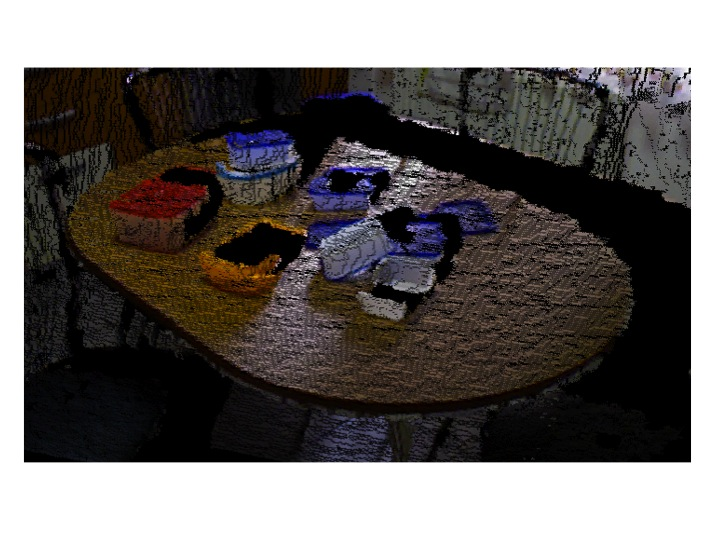
\includegraphics[scale = 0.3]{figures/Slide02.jpg}
\caption{An example of the noise from a Kinect-like sensor}
\vspace*{-10pt}
\label{fig:noisy data}
\end{figure}


\section{Related Work}

While a variety of grasp metrics have been proposed, few explicitly looked at uncertainty in grasp parameters. Zheng et al. looked at friction and contact point uncertainty \cite{zheng2005}. He computed the maximum distance a contact point was allowed to deviate from its expected grasp, while maintaining force closure. Kehoe et al. looked at shape uncertainty for push grasps, however this was limited to parallel jaw grippers and only measured the probability of force closure \cite{kehoe2012toward}. More closely related to our approach is the work of Christopoulos and Schrater \cite{christopoulos2007handling}. They use a spline representation for uncertainty and sample from a distribution of losing force closure, their approach though is limited to two contacts. Our method looks at not only force closure, but provides a lower bound on the Ferrari-Canny metric within some user set distributions.  

The choice of using a Gaussian Process Implicit Surface (GPIS) to represent our uncertainty, stems from the fact that it provides a formal way to include various sources of noise in observations. Prior work has used uncertainty representation such as independent Gaussian noise on each vertex in a Polygonal mesh \cite{kehoe2012toward}. However, this doesn't provide a continuous function one can easily compute distributions on grasp parameters with. GPIS is also becoming more prevalent in the grasping community with recent work by Dragiev et al. \cite{dragiev2011} . 



\section{Gaussian Process Implicit Surfaces}

In this section we describe the mathematical derivation of Gaussian Process Implicit Surface representations.

\subsection{Gaussian Process (GP) Background}

Gaussian processes (GPs) are widely used in machine learning as a nonparametric regression method for estimating continuous functions from sparse and noisy data \cite{rasmussen2006gaussian}.
In a GP, a training set consists of input vectors $\mX = \{\bx_1, \ldots, \bx_n\}$, $\bx_i \in \mathbb{R}^d$, and corresponding observations $\by = \{y_1, \ldots, y_n\}$. The observations are assumed to be noisy measurements from the unknown target function $f$:
\begin{equation}
y_i = f(\bx_i) + \epsilon,
\end{equation}
where $\epsilon \sim \mN(0,\sigma^2)$ is Gaussian noise in the observations.
A zero-mean Gaussian process is completely specified by a covariance function $k(\cdot,\cdot)$, also referred to as a kernel.
Given the training data $\mD = \{\mX, \by\}$ and covariance function $k(\cdot,\cdot)$, the posterior density $p(f_*|\bx_*,\mD)$ at a test point $\bx_{*}$ is shown to be \cite{rasmussen2006gaussian}:
\begin{align}
	p(f_*|\bx_*,\mD) &\sim \mN\big(\mu(\bx_*), \Sigma(\bx_*)\big) \label{eq:GPposterior} \\
	\mu(\bx_*) &= k(\mX,\bx_*)^{\intercal}(K + \sigma^2I)^{-1}\by \label{eq:GPmean} \\
	\Sigma(\bx_*) &= k(\bx_*,\bx_*)-k(\mX,\bx_*)^{\intercal}(K+\sigma^2I)^{-1}k(\mX,\bx_*)\big) \label{eq:GPvar}
\end{align}
where $K \in \mathbb{R}^{n \times n}$ is a matrix with entries $K_{ij} = k(\bx_i,\bx_j)$ and $k(\mX,\bx_*) = [k(\bx_1,\bx_*),\ldots,k(\bx_n,\bx_*)]^{\intercal}$. 
This derivation can also be used to predict the mean and variance of the function gradient by extending the kernel matrices using the identities \cite{solak2003derivative}:

\begin{align*}
	\text{cov}\left(f(\bx_i), f(\bx_j) \right) &=  k(\bx_i, \bx_j) \\
	\text{cov}\left(\frac{\partial f (\bx_i)}{\partial x_k}, f(\bx_j) \right) &= \frac{\partial}{\partial x_k} k(\bx_i, \bx_j) \\
	\text{cov}\left(\frac{\partial f (\bx_i)}{\partial x_k}, \frac{\partial f (\bx_j)}{\partial x_l} \right) &= \frac{\partial^2}{\partial x_k \partial x_l} k(\bx_i, \bx_j)
\end{align*}

\subsection{Kernel Selection}
The choice of kernel is application-specific, since the function $k(\bx_i,\bx_j)$ is used as a measure of correlation between states $\bx_i$ and $\bx_j$. A common choice is the squared exponential kernel:
\begin{equation}
	k(\bx_i,\bx_j) = \nu^2\exp(-\frac{1}{2}(\bx_i - \bx_j)^{\intercal}\Lambda^{-1}(\bx_i - \bx_j))
\end{equation}
where $\Lambda= \text{diag}(\lambda_1^2,\ldots,\lambda_d^2)$ are the characteristic length scales of each dimension of $\bx$ and $\nu^2$ describes the variability of $f$.
Other common kernels relevant to GPIS are the thin-plate splines kernel \cite{williams2007} and the Matern kernel \cite{bjorkman2013enhancing}.

The measurement noise parameter $\sigma$ is usually estimated based on a model of the sensor used to collect measurements
The vector of remaining hyperparameters $\boldsymbol{\theta} = \{\nu, \lambda_1,\ldots,\lambda_d\}$ is optimized during the training process by maximizing the log-likelihood $p(\by|\mX,\boldsymbol{\theta})$, usually using gradient descent \cite{rasmussen2006gaussian}.
The log-likelihood function is subject to local maxima, and therefore the hyperparamter search often involves a search over the maxima found from several random initializations of the hyperparamters.

\subsection{Training}
Given the hyperparameters, the training phase consists of evaluating the vector 
\begin{equation}
\alpha = (K + \sigma^2 I)^{-1}\by,
\end{equation}
which needs the inversion of a $n \times n$ matrix $(K + \sigma^2I)$. Direct computation of the inverse of the symmetric matrix requires $O(n^3)$ operations and $O(n^2)$ storage, which makes it impractical for real-world applications consisting of thousands of data points.

For larger systems, it is more efficient to solve the system
\begin{equation}
	\tilde{K}\alpha = \by, ~\text{where} ~\tilde{K} = (K + \sigma^2I),
\end{equation}
using iterative methods. Since $\tilde{K}$ is symmetric and positive-definite, the conjugate gradient (CG) method or an incomplete Cholesky factorizatoin can be used to iteratively solve the equation to some error tolerance \cite{gibbs1997}.
The computational complexity of the CG method is $O(kdn^2)$ where $d$ is the dimensionality of the data and $k$ iterations of the CG method are required for convergence.
Fast approximate matrix-vector products using the Improved Fast Gaussian Transform (IGFT) can reduce the complexity of computing the $\alpha$ vector to $O(n)$ for the squared exponential kernel \cite{raykar2007}.
Alternatively Fast Multipole Methods can be used to reduce the complexity of computing the kernel matrices and vectors to $O(n \log n)$ \cite{gumerov2005fast}.

A large variety of methods haven been proposed for further speeding up the GP training phase including, but not limited to, training on a subset of data chosen either randomly or using an information-theoretic criterion, or local methods that only rely on neighboring data points for making predictions in a given region of space.
The subset selection methods can be separated into two groups: subset of data (SoD) and subset of regressors (SoR) \cite{quinonero2005unifying}.
In SoD approaches, a criterion is used to select an `active' subset of training data to be used in inference, and all other `inactive' training data is discarded.
In SoR approaches the relation of the inactive points to the active points is retained by replacing the kernel function with the alternative function
\begin{equation}
	k(\textbf{x}_i,\textbf{x}_j) = k(\textbf{x}_i,\textbf{u}) K_{\textbf{u}, \textbf{u}}^{-1} k(\textbf{u},\textbf{x}_j).
\end{equation}
\noindent We refer the reader to \cite{chalupka2013} for an extensive comparison of these methods. In this paper we consider objects that can be represented with few enough points that computational tractability is not an issue, and we defer the question of which methods are most effective for the special case of constructing GPIS to future work.

\begin{figure}[ht!]
\centering
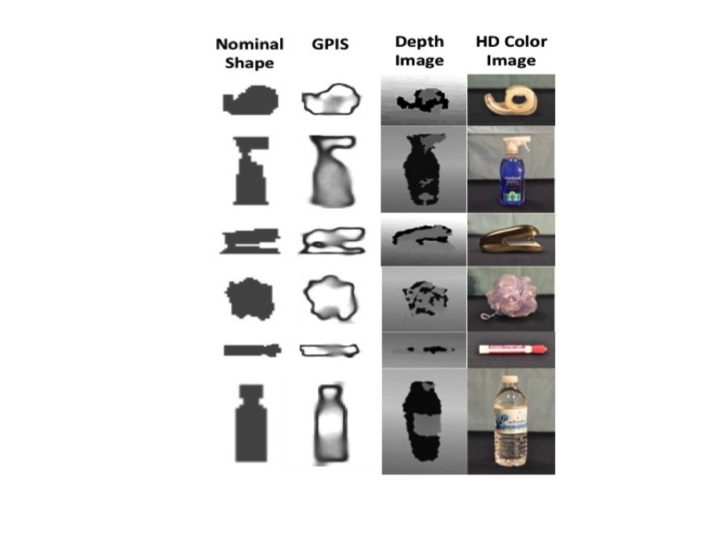
\includegraphics[scale = 0.3]{figures/Slide03.jpg}
\caption{Left: A surface represented as a Truncated Signed Distance Field (TSDF).
Right: A GPIS reconstruction from noisy samples of the left surface's TSDF.}
\vspace*{-10pt}
\label{fig:GPIS_TSDF}
\end{figure}
%\section{Related Work}

\section{Problem Definition}

The objective of our algorithm is to provide a quality of the expected grasp, $Q_l^-(\bar{g})$ \cite{ferrari1992}, and a lower bound $b$ that is the expected deviation from the quality of the expected grasp. 

We assume a bounded rectangular workspace $\mathcal{R}$.
We parameterize a given grasp $g$ on an object with the following tuple $g = \lbrace \textbf{c}_1,...,\textbf{c}_m,\textbf{n}_1,...,\textbf{n}_m,\textbf{z},\tau\rbrace$.
We have an indexing set $I$ of $m$ point contacts and surface normal on the object: for $i \in I$ the contact is located at $c_i$ with surface normal $n_i$.
The object has a center of mass $z$ and friction coefficient $\tau$.
The line segment $\gamma(\cdot)$ has endpoints $a,b$ that are defined as the start of the gripper and the intersection of the line with the end of the workspace respectively, as shown in Fig. 
 \ref{fig:line_of_action}.


Since we have uncertainty in the shape we have a distribution on the grasp parameters, hence $p(g) = \lbrace p(\textbf{c}_1),...,p(\textbf{c}_m),p(\textbf{n}_1),...,p(\textbf{n}_m),\bar{\textbf{z}},\tau \rbrace$.
We note that $\tau$ is considered known and $\bar{z}$ is only the expected center of mass, not a full distribution. In section \ref{sec:distgrasp}, we demonstrate how to efficiently compute these distributions on contact points and surface normals. 

With a distribution on $p(g)$ we then aim to use recent results on a Lipschitz constant for the Ferrari-Canny Metric \cite{pokorny2013classical} to provide $b$ or a lower bound on the change in grasp quality from the expected deviation in grasp and the quality of the expected grasp $Q_l^-(\bar{g})$, where $\bar{g} = \lbrace \bar{\textbf{c}}_1,...,\bar{\textbf{c}}_m,\bar{\textbf{n}}_1,...,\bar{\textbf{n}}_m,\bar{\textbf{z}},\tau \rbrace$.



\section{Distribution of Grasp Parameters}
\label{sec:distgrasp}

 For the following derivations we introduce the following,
 $\theta(x) = \lbrace \mu(x),\Sigma(x) \rbrace$, where $\theta(x)$ is a tuple consisting of the mean and covariance functions given by the trained GPIS model \cite{rasmussen2006} . 
 
 To calculate $p(g)$, we assume a gripper contacts approaches along a parameterized line of action, or a 1-dimensional curve in the work space, defined by $\gamma(t)$. See Fig \ref{fig:line_of_action}, for a detailed illustration. Each gripper contact is defined by a line of action, so we assume the following tuple is provided $\Gamma = \lbrace \gamma_1(\cdot),...,\gamma_m(\cdot) \rbrace$, these approach trajectories are then used to compute a distribution on grasp parameters. 
 



 %We also define the  level set function as $f(x): \mathbb{R}^d \rightarrow \mathbb{R}$ and an implicit surface as $\mathcal{S} = \{ x \ | \ f(x) = 0 \}$.


\begin{figure}[ht!]
\centering
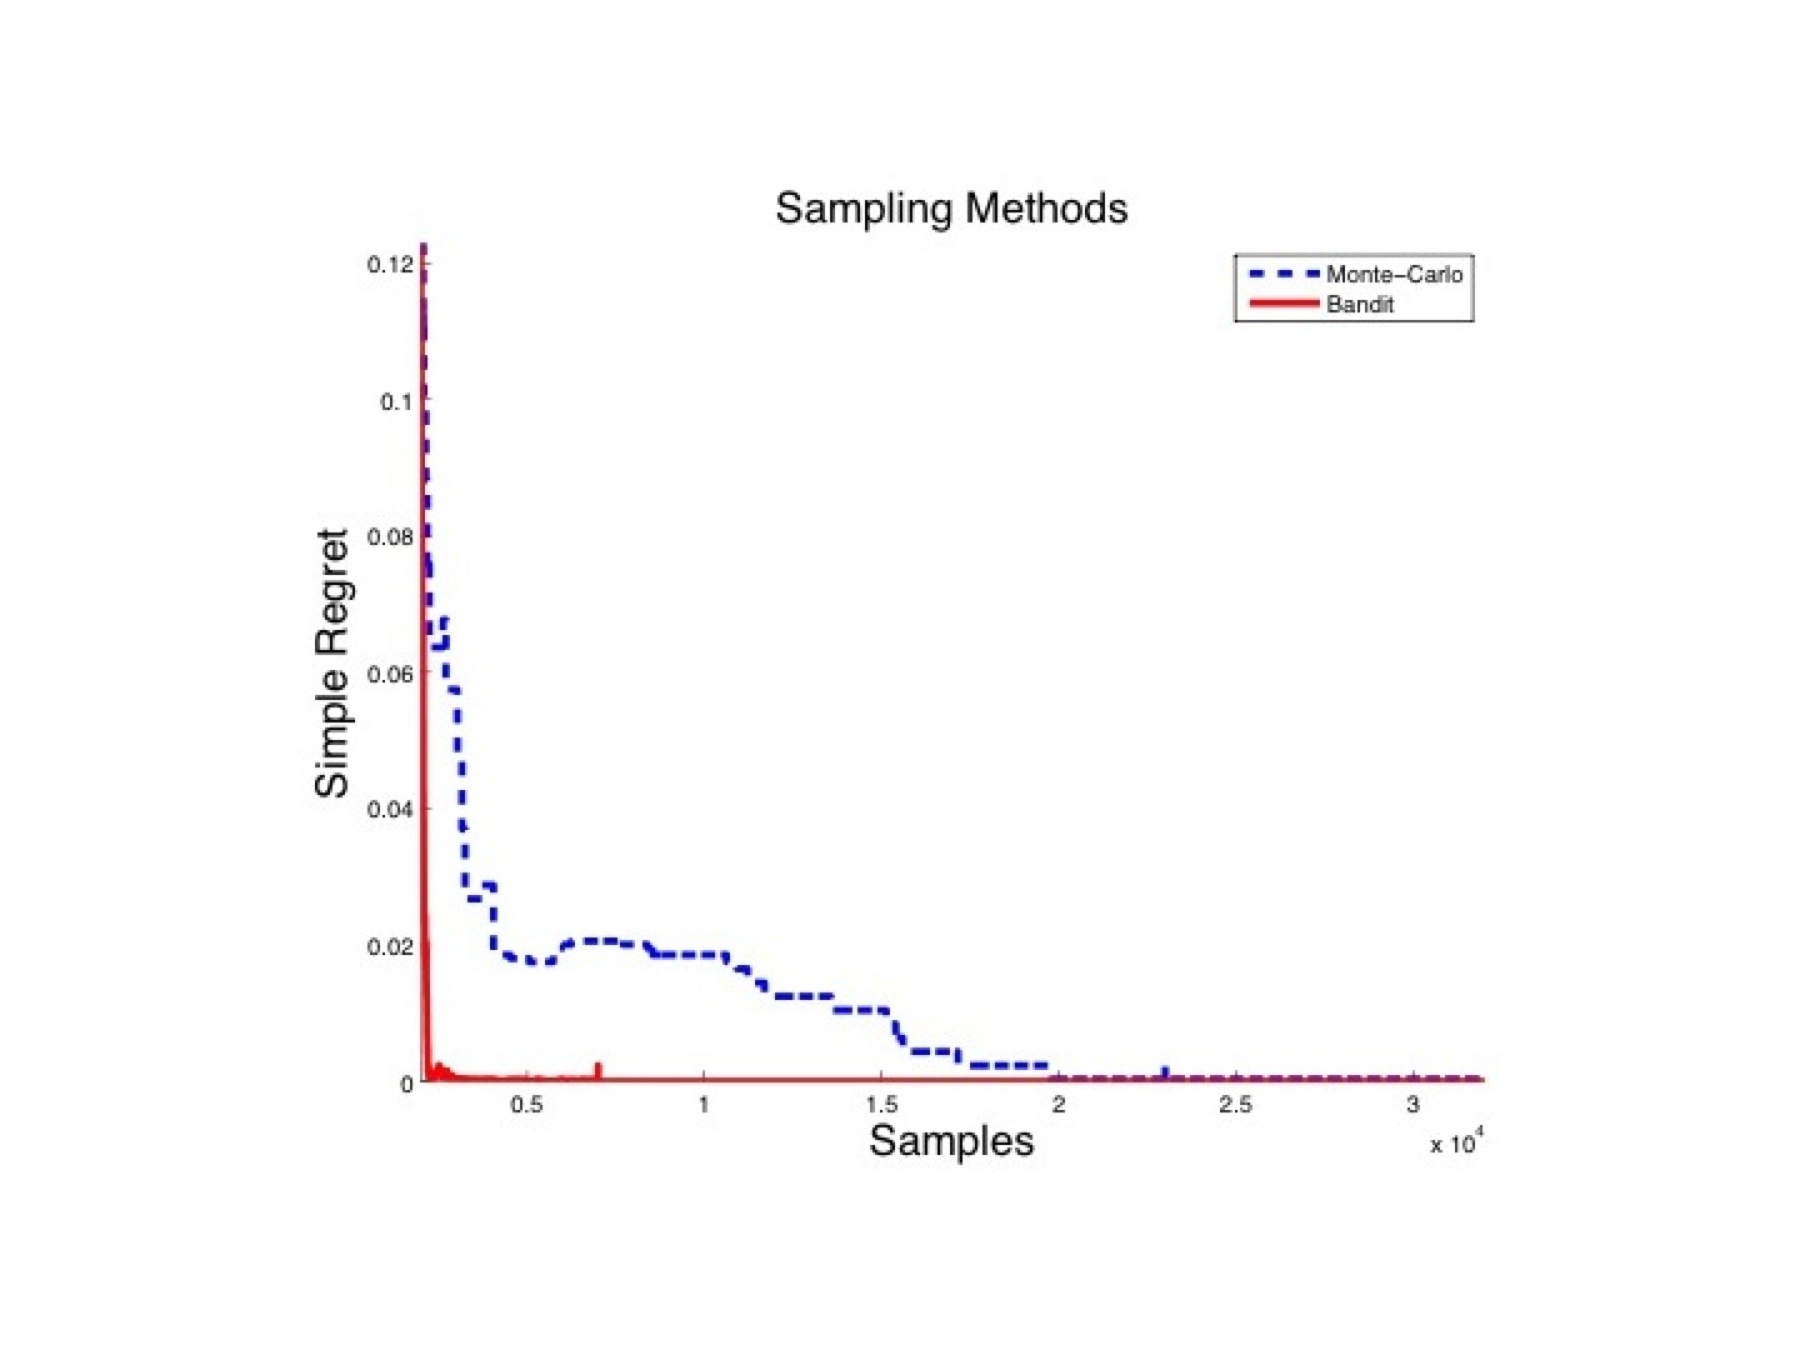
\includegraphics[scale = 0.3]{figures/Slide01.jpg}
\caption{Parameterized Line of Action along an object}
\vspace*{-10pt}
\label{fig:line_of_action}
\end{figure}
%\textbf{TODO:MORE DESCRIPTIVE GRAPHIC}
\subsection{Distribution on Contact Points} 
In our implementation we discretize along the line $\gamma(t)$ evenly but write the derivation in continuous form for generality.
The probability distribution along the line $\gamma(t)$ is given by the following:

\begin{equation}
p\big(f(\gamma(t))|\theta(\gamma(t)): \forall t \in [a,b] \big) 
=
\mN(\mu_{a:b},\Sigma_{a:b}).
\end{equation}

This gives the signed distance function distributions along the entire line of action in the workspace as a multivariate gaussian.
We would like to find the distribution on the first contact point, which we can define as when the signed distance function $f(\gamma(t))$ is $0$ and all previous times $\tau$ we have $f(\gamma(\tau)) > 0$ for $0 \leq \tau < t$.
This ensures $t$ is at the edge of the surface (having $f(\gamma(t)) = 0$) and that for all previous $\tau$ the gripper was outside of the surface (having $f(\gamma(\tau)) > 0$).
We thus compute this as the joint distribution $p\big(\textbf{c}_i= \gamma(t)\big) = p\big(f(\gamma(t))=0, f(\gamma(\tau))> 0: \forall \tau \in [0,t)\big)$.
%Hence we want to know at a point what the distribution  is that it is at the surface and the probability that all points before are before the surface,
This avoids the problem of the distribution producing multiple modes along the line: one for each intersection with the surface.
We now derive this distribution 

\begin{align*}
p\big(\textbf{c}_i = \gamma(t)\big) &\propto p\big(f(\gamma(t)) = 0\big)\\
               &*P\big(f(\gamma(\tau)) > 0 | f(\gamma(t)) = 0: \forall \tau \in [0,t)\big)
\end{align*}

where we only indicate proportionality and will later normalize to probability $1$.
Using the first product in the equation can be computed easily using the marginalization of a multivariate Gaussian distribution and the second one can be rewritten by conditioning the distribution \cite{petersen2008matrix}. 

\begin{align*}
p_c\big(f(\gamma(\tau)): \forall \tau \in [0,t)\big) = p\big(f(\gamma(\tau))  | f(\gamma(t)) = 0\big)  
\end{align*}


The following can now be said:

\begin{align*}
p\big(\textbf{c}_i = \gamma(t)\big) &= \frac{1}{\eta} p(f\gamma(t) = 0) \\
				   &*P_c\big(f(\gamma(\tau)) > 0): \forall \tau \in [0,t)\big)			 
\end{align*} 

for the appropriate $\eta$ normalization factor.
The second product term can be evaluated by calculating the cumulative distribution of a multivariate Gaussian, which we calculate with the Matlab function $mvncdf$.
We show again the theoretical distribution on $\textbf{c}_i$ calculated for a given GPIS and approach direction in Fig.
\ref{fig:GraspContactPt}.
%efficiently evaluated by looking up the cumulative distribution of a multivariate Gaussian, which is common in most software packages \cite{matlab}.

\begin{figure}[ht!]
\centering
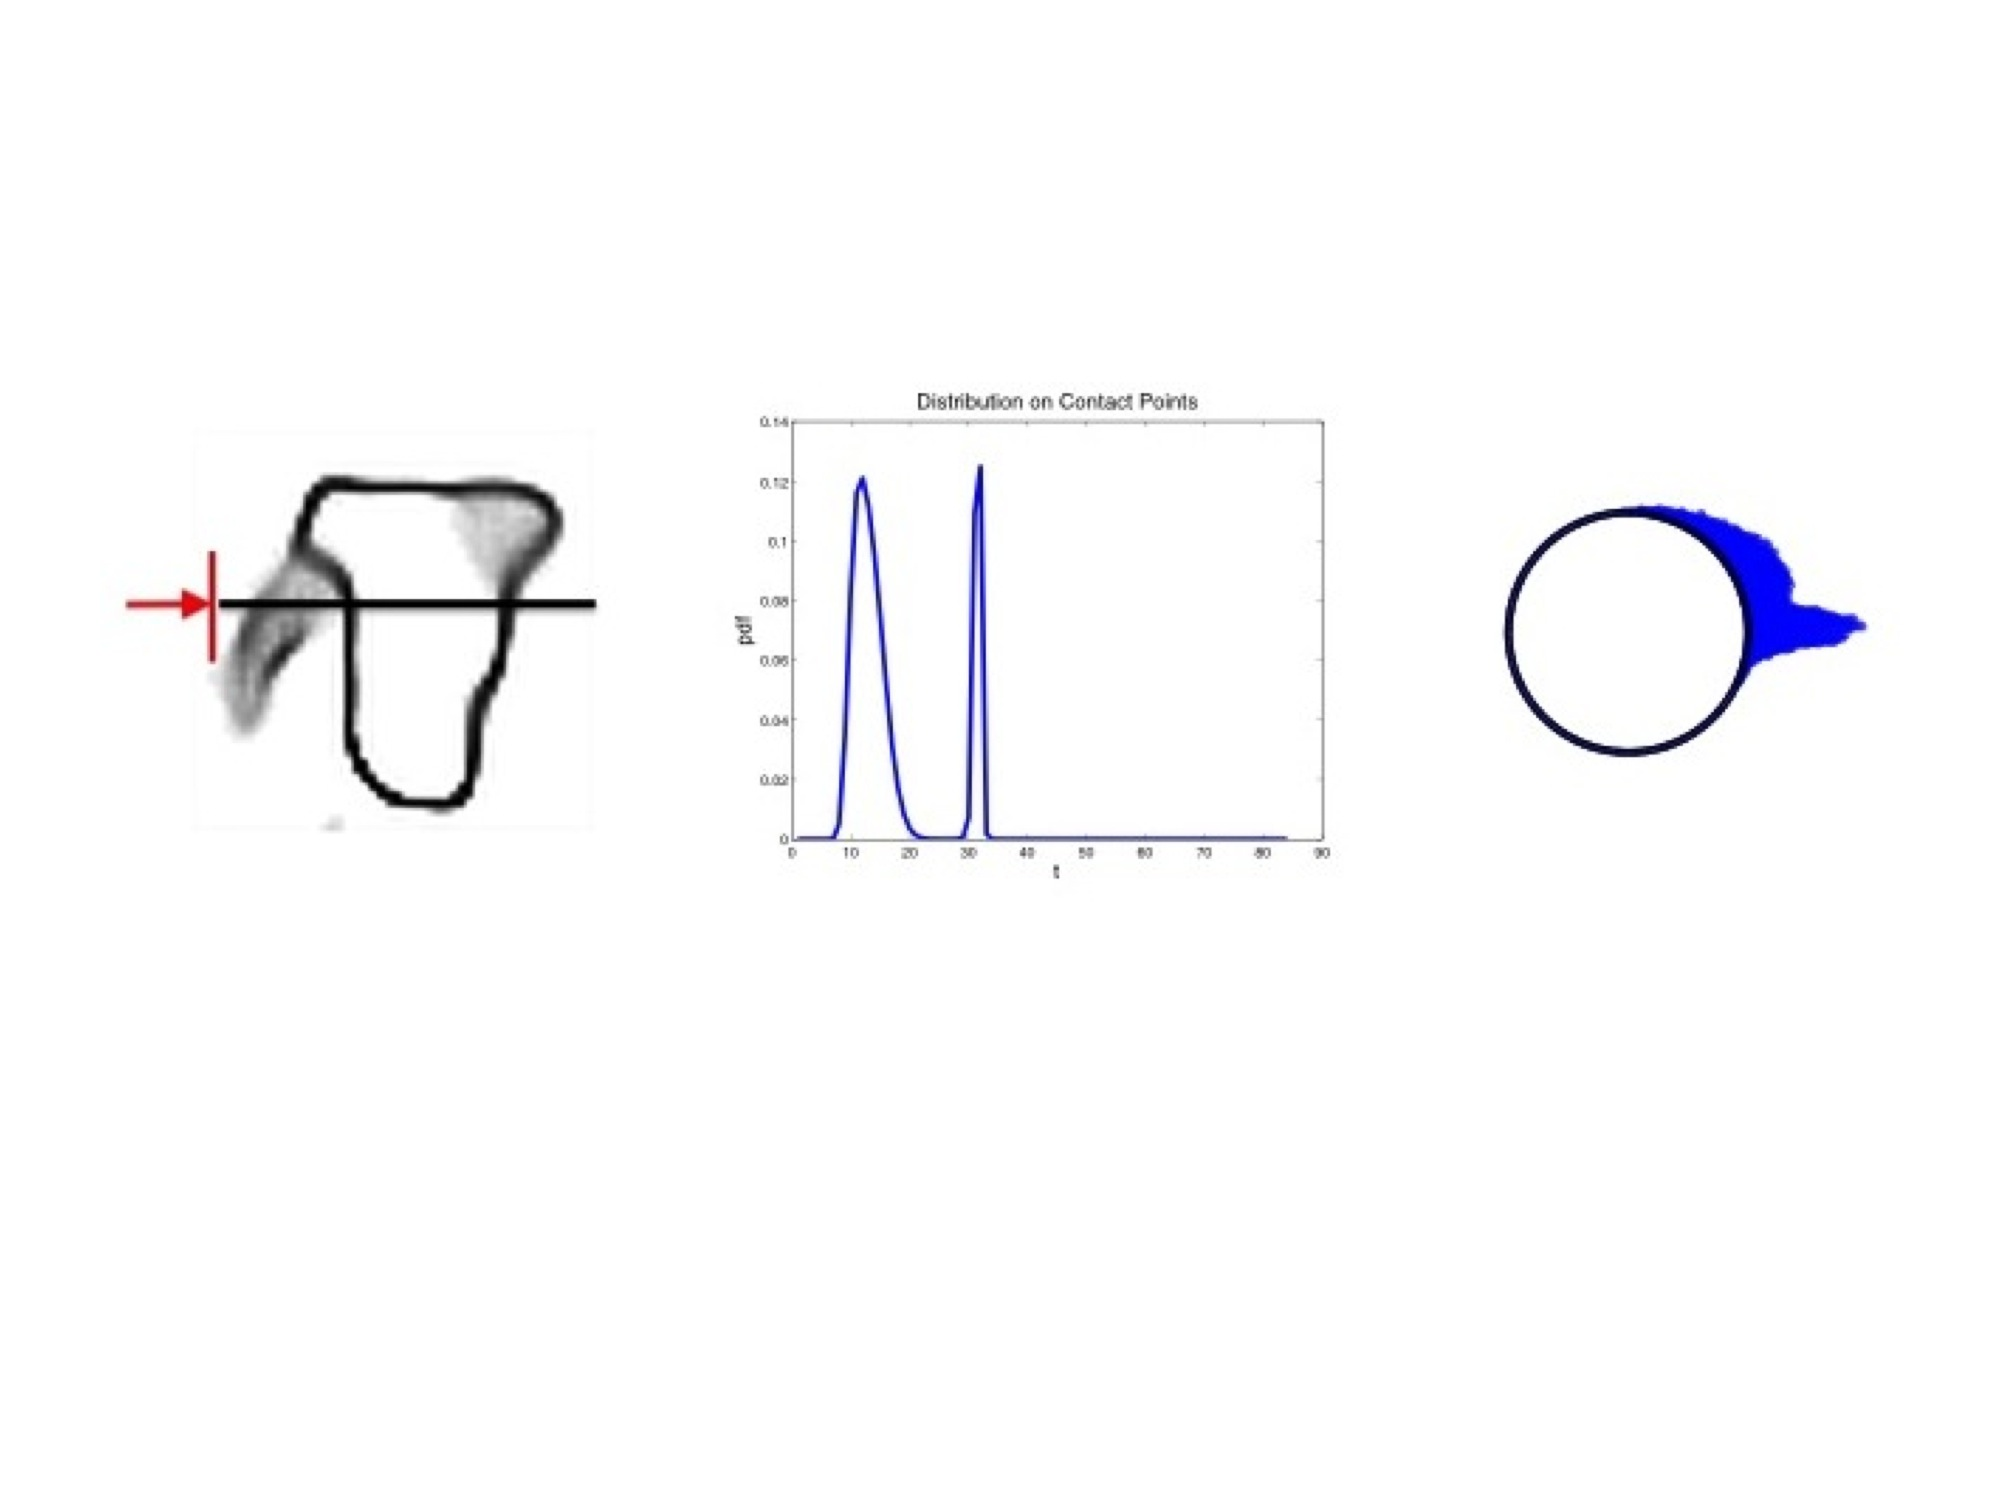
\includegraphics[scale = 0.3]{figures/Slide04.jpg}
\caption{Left: Grasp approach direction on an uncertain surface, represented by a Gaussian Process Implicit Surface.  Right: Induced distribution on the contact point as a function of x-axis position along the approach line.}
\vspace*{-10pt}
\label{fig:GraspContactPt}
\end{figure}

\subsection{Distribution on Surface Normals} 
The distribution of surface normals $p(\textbf{n}_i = \textbf{k})$ can be calculate as follows.
First we assume that some function exists $h(x) = \lbrace \mu_{\nabla}(x), \Sigma_{\nabla}(x) \rbrace$, hence given a point $\bf{x}$ it returns the parameters for a Gaussian distribution around the gradient.
this function can be computed via learning the gradient \cite{solak2003derivative} or analytical differentiation of $f(x)$.
We note that both methods yield a Gaussian distribution.
We now demonstrate how to marginalize out the contact distribution and compute $p(\textbf{n}_i = \textbf{k})$.\\

From our distribution on contact points and Bayes rule we can compute the following: 

\begin{equation}
p(\textbf{c}_i = \gamma(t), \textbf{n}_i = \textbf{k}) = p\big(\textbf{n}_i = \textbf{k} | \textbf{c}_i = \gamma(t) \big)*p\big(\textbf{c}_i = \gamma(t)\big)
\end{equation}

Now we can marginalize out the distribution on contacts:

\begin{equation}
p(\textbf{n}_i = \textbf{k}) = \int_a^b  p \big(\textbf{n}_i = \textbf{k} | \textbf{c}_i = \gamma(t) \big)*p(\textbf{c}_i = \gamma(t)) dt
\end{equation}

\begin{equation}
p\big(\textbf{n}_i = \textbf{k}\big) = \int_a^b  p \big(\textbf{n}_i = \textbf{k} | h(\gamma(t))\big)*p\big(\textbf{c}_i = \gamma(t)\big) dt
\end{equation}

We approximate this by uniformly sampling the integral along the function $\gamma(t)$ and achieve the following: 

\begin{equation}
p\big( \textbf{n}_i = \textbf{k} \big) = \sum_T  p \big( \textbf{n}_i = \textbf{k} | h(\gamma(t)) \big) *p\big(\textbf{c}_i = \gamma(t)\big) \Delta t
\end{equation}


The traditional grasp metrics, such as  Ferrari-Canny, requires $\textbf{n}_i$ be normalized, or, equivalently, a member of $\mathcal{S}^{d-1}$ \cite{ferrari1992}. To account for this we project the Gaussian distribution $p \big(\textbf{n}_i = \textbf{k} |\textbf{c}_i = \gamma(t) \big)$  onto $\mathcal{S}^{d-1}$. We use a stereographic projection technique developed by Olano and North \cite{olano1997normal}. In Fig.6
\ref{fig:GraspSurfaceNormals}, we show the theoretical distribution on $\textbf{n}_i$ calculated for a given GPIS and approach direction .

\begin{figure}[ht!]
\centering
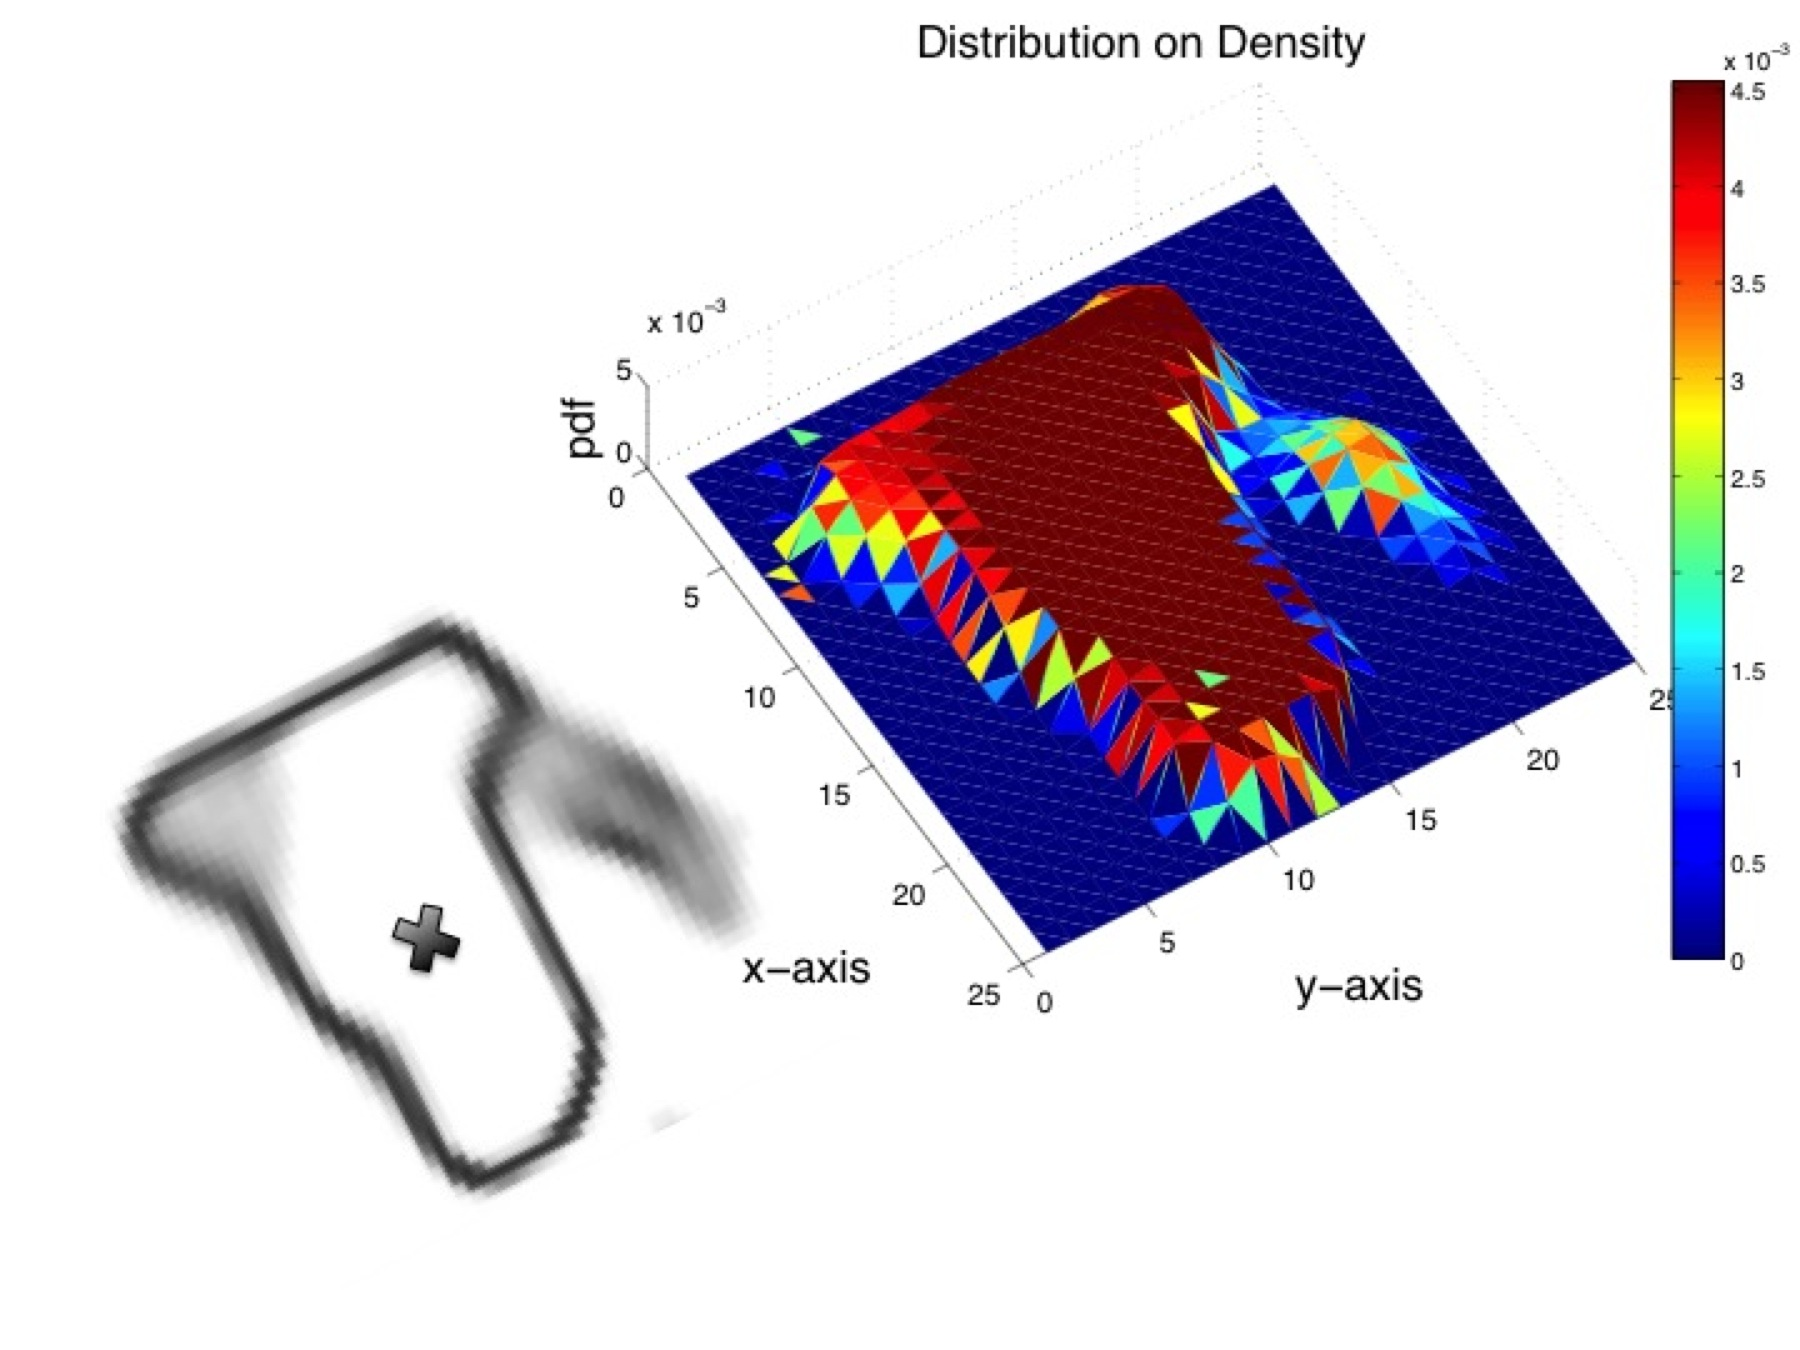
\includegraphics[scale = 0.3]{figures/Slide05.jpg}
\caption{Left: Grasp approach direction on an uncertain surface, represented by a Gaussian Process Implicit Surface.
Right: Induced distribution on the surface normals.}
\vspace*{-10pt}
\label{fig:GraspSurfaceNormals}
\end{figure}

\subsection{Expected Center of Mass} 

We define the quantity $\mathcal{D}(x) = \int_{-\infty}^{0} p(f(x) =  s \ | \ \theta(x)) ds$ and note that it is equal to the probability that x is interior to the surface under the current observations.
$\mathcal{D}(x)$ can be calculated as the CDF of $f(x)$ at $0$.
We assume that the object has uniform mass density and then $\mathcal{D}(x)$ is the expected mass density at x.
Then we can find the expected center of mass as:

\begin{equation}
  \bar{z} 
  =
  \frac
    {\int_{\mathcal{R}}x \mathcal{D}(x) dx}
    {\int_{\mathcal{R}}  \mathcal{D}(x) dx}
\end{equation}

which can be approximated by sampling $\mathcal{R}$ uniformly in a voxel grid and approximating the spatial integral by a sum. We show the computed density and caculated expected center of mass in Fig. \ref{fig:GPIS_MASS}.


\begin{figure}[ht!]
\centering
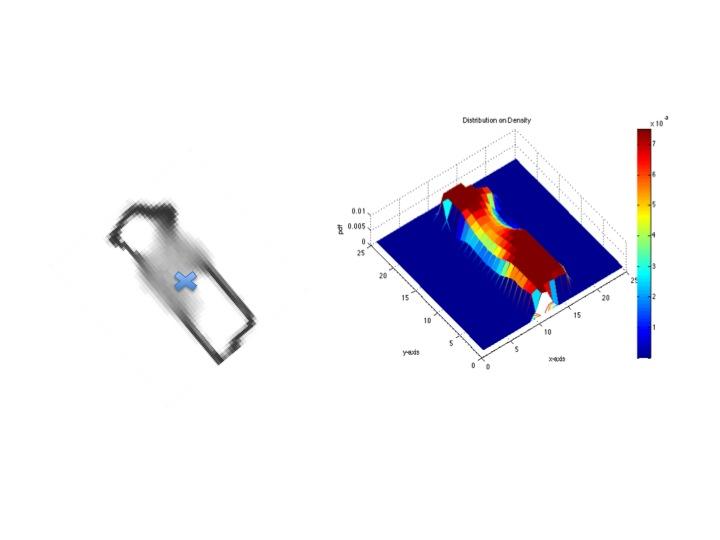
\includegraphics[scale = 0.3]{figures/Slide06.jpg}
\caption{Left: A surface with GPIS construction and expected center of mass (blue X)
Right: The distribution on the density of each point assuming uniform center of mass}
\vspace*{-10pt}
\label{fig:GPIS_MASS}
\end{figure}

\section{Probabilistic Bound on Grasp Metric}
\label{sec:bound}
Following recent work on proving a Lipschitz bound on the Ferrari-Canny Metric \cite{pokorny2013classical}, we would like to prove an extension to give a probabilistic bound on the change in grasp quality.
We restate several of their results here:

\subsection{Derivation of Lipschitz Constant }

We follow the notation of \cite{pokorny2013classical} except that their $\mu$ is our $\tau$ since we use $\mu$ to refer to means.  
We re-state some of their central theorems for our use here.
For more detail, refer there.
$Q(g)$ is the exact $L^1$ grasp quality.
It is denoted by the following 

\begin{align}
  Q(g) &= \mbox{max}(0,q(g)) = -d(0,\mbox{Conv}(\{0\} \cup S(g))\\
-d(0,S) &= min_{||z|| = 1} h_{S(z)}\\
h_{S(z)} &= \mbox{sup}_{s\in S}\langle s,z\rangle\\
\end{align}

We denote the Ferrari-Canny version, which approximates the friction cone by a linearized set of wrenches\cite{ferrari1992}, as $Q^-_l(g)$.
The next theorem shows that the linearized wrench set used in Ferrari-Canny calculates a lower bound on $Q(g)$.\\

\begin{theorem}
  \cite{pokorny2013classical}
For any grasp g, we have $0 \leq Q_l^-(g) \leq Q(g)$.
Furthermore, $||Q(g) - Q^-_l(g)|| \rightarrow 0$ as $l \rightarrow \infty$ when $Q_l^-(g)$ is computed using a uniform approximation of the friction cones with $l$ edges. \\
\end{theorem}

The next theorems are used to show that $Q$ is Lipschitz continuous.

\begin{theorem}
\label{lemma35}
  \cite{pokorny2013classical}
For $w \in \mathbb{R}^3$, we have, for $n \in \mathbb{S}^2$ and for friction coefficient $\mu > 0$, 

\begin{align}
\mbox{sup}_{x \in C(n)} \langle x,w \rangle = \langle n,w \rangle + \tau||n \times w||
\end{align}

Hence, for $u = (a,b) \in \mathbb{R}^3 \times \mathbb{R}^3 = \mathbb{R}^6$, we have 

\[
h_{W_i(g)}(a,b) =
 \langle n_i,a+b\times(c_i-z)\rangle +
\]
\begin{align}
 +\tau ||n_i \times (a+b\times(c_i-z))||
\end{align}

\end{theorem}

\begin{theorem}
  \cite{pokorny2013classical}
We have \\

\begin{align}
q(g) 
=
\min_{u\in \mathbb{R}^6, ||u|| =1} h_{S(g)}(u) 
=
\end{align}
\[
\min_{u\in \mathbb{R}^6, ||u|| =1} \max_{i=1,...,m} h_{W_i(g)}(u),
\]

where $h_{S(g)}$ is convex on $\mathbb{R}^6$.
$q$ is invariant under fixed translation of the grasp center and contact positions.
Furthermore, let $\mathbb{B}(r) = \lbrace x \in \mathbb{R}^3 : ||x|| \leq r \rbrace$.
Then $q$ is Lipschitz continuous on grasps with $m$ contact points lying in the set $X = \lbrace (c_1, \dots, c_m,n_1, \dots,n_m,z) : (c_i-z) \in \mathbb{B}(r), n_i \in \mathbb{S}^2 \rbrace$ with a Lipschitz constant given by $L= (1+\mu)(1+r)$ and where we use distance measure 

\[
  d(g,g') = \sum_i ||(c_i-z)-(c_i'-z')|| + \sum_i ||n_i - n_i'||.
\]

We hence have 

\[
|q(g) - q(g')| \leq Ld(g,g'),\  \forall g,g' \in X.
\]

Since $Q(g) = \max(0,q(g))$, $Q$ is also Lipschitz continuous with the same constant $L$ on $X$. 
\end{theorem}

Setting $l_{i,a,b} = h_{W_i(g)}(a,b)$, we have for $||(a,b)|| \leq 1$ that is $|l_{i,a,b}(g) - l_{i,a,b}(g')|$ is bounded by $|\langle n_i,a+b\times (c_i-z)\rangle - \langle n_i',a+b\times(c_i'-z')\rangle|+\mu|||n_i \times (a+b \times (c_i -z))|| - ||n_i \times (a + b \times (c_i' - z')) |||$, using Theorem \ref{lemma35}.
By using the following facts $||a|| \leq 1$, $||b|| \leq 1$, $||v \times w || \leq ||w||||v||$, $|\langle v,w\rangle | \leq ||v||||w||$, we obtain:  

\begin{align*}
|l_{i,a,b}(g) - l_{i,a,b}(g')| &\leq ||n_i - n_i'||(1+||c_i - z||) \\
					&+ ||(c_i - z)-(c_i'-z')|| \\
					&+ \tau(||n_i - n_i'||(1+||c_i - z||)\\
					&+||(c_i - z)-(c_i'-z')||)
\end{align*}

\subsection{Lower Bound on Expected Grasp Quality}
Given a the distributions on a line of action, $p\big(\textbf{n}_i = \textbf{k}\big)$ and $p\big(\textbf{c}_i=\gamma(t) \big)$ and the expected values $\bar{\textbf{c}_i}$ and $\bar{\textbf{n}_i}$. We are interested in finding the expected deviations for the two parameters, $||\Delta n_i||$ and  $||\Delta c_i||$. Using these expected deviations we then derive a lower bound $b$ for the quality of the expected grasp. 

\[
  ||\Delta n_i|| =  \int_{\mathbb{B}(\bar{\textbf{n}_i})} ||\textbf{k} - \bar{\textbf{n}_i}|| p(\textbf{n}_i = \textbf{k}) d\textbf{k}
\]

\[
  ||\Delta c_i|| =  \int_{\mathbb{B}(\bar{\textbf{c}_i)}} ||\gamma(t) - \bar{\textbf{c}_i}|| p(\textbf{c}_i = \textbf{k}) dt
\]

We now write the above bound as follows for a given line of action $i$: 

 \begin{align*}
|l_{i,a,b}(g) - l_{i,a,b}(g')| & \leq (1+\tau)||\Delta \textbf{n}_{i}||(1+||\bar{\textbf{r}}_i||) + ||\Delta{\textbf{c}_{i}}|| \\
  \end{align*}

Here $\bar{\textbf{r}}_i = \bar{\textbf{c}}_i - \bar{\textbf{z}}_i$. For convenience we rewrite the bound on a given set of grasp parameters as : 

 \begin{align*}
b_i &= (1+\tau)||\Delta \textbf{n}_{i}||(1+||\bar{\textbf{r}}_i||) + ||\Delta{\textbf{c}_{i}}|| \\
\end{align*}

To provide an upper bound overall contact parameters we introduce the following: 

\begin{align}
b(\zeta)  = \max_{i} b_i(\zeta)
\end{align}

To prove if  this bound is preserved on

 \begin{align}
 q(g) = \min_{(a,b) \in \mathbb{R}^6, ||u||=1} \max_{i=1,..,m} l_{i,a,b}(g)
 \end{align}
 
we turn to the general case.
$\lambda(x) = \mbox{inf}_{\alpha \in A} f_\alpha(x)$ and $\lambda(x) = \mbox{sup}_{\alpha \in A} f_\alpha(x)$ are bounded with $b(\zeta)$ if $f_\alpha(x)$ for all $\alpha$ is bounded with $b(\zeta)$ and $\lambda(x)$ is bounded.
Since our bound is invariant to the variables $(a,b)$ and we take the maximum set of parameters $i$.
We can ensure that is true.


\subsection{Tightening Bounds on Change in Grasp Quality}

Experimentally we found the Lipschitz bound to be looser than we would like, despite the fact that it is a local bound. We are currently working on tightening the bound by using the following property: 

For a $x,x_0$ in a bounded set $U$ in $\mathbb{R}^n$, for a given $f(x):\mathbb{R}^n \rightarrow \mathbb{R}$. 

\[
  f(x) = f(x_0) + \langle R(x),x-x_0 \rangle
\]

\[
  R(x) = \int_0^1 \frac{d}{dx}f(x_0+t(x-x_0)) dt
\]

Then let $L = \mbox{sup}_{s \in U} |\frac{df(x)}{dx} |$, so $|R(x)| \leq L$ and 

\[
  |f(x)-f(x_0)| = |\langle R(x),x-x_0 \rangle| \leq L |x-x_0|
\]


Since we are currently working in 2D, there is no need to approximate the friction cone and the Ferrari-Canny is equal to the true grasp quality. What that means is that one could look at the analytical derivative of the active facet and use that to bound the metric. Looking at a single facet on the convex hull computed by Ferrari-Canny, one simply computes the derivative of the function $h(W,\textbf{z},\tau)$, where $h$ returns the absolute distance to the origin $d$ from the facet described by the input parameters. 

While we can compute the derivative using symbolic software \cite{SymPy}, it is still on going work to quickly determine either the set $U$ that the bound is valid or supremum of the derivative in a given set.    

\subsection{Approximation of True Metric}
While we work on the tightening the bound, we will present a metric that should give an intuitive idea of what is import in our grasp metric. Our grasp metric currently returns $Q(\bar{g})$ and an upper bound $b$ on the expected change in grasp. Ideally we want to rate grasps by the highest value $Q_l = Q(\bar{g}) - b$, thus being the lowest quality given the bound. 

Currently though the two values $Q(\bar{g})$ and $b$ are two different magnitudes, but both are informative. We can approximate a the effect of a tighter bound by simply projecting both $Q(\bar{g})$ and $b$ to the unit ball, then subtracting. 

\section{Experiments}

To validate our theoretical caculations, we compared them to empirical distributions found via Monte-Carlo Sampling. The qualitative results for surface normals and contacts can be found in Figures \ref{fig:Contact_Dist} and \ref{fig:Normal_Dist} respectively. We present the numerical comparison with KL-Divergence in Table 1, as you can see the distributions are very closely related. 

\begin{table}[ht!]
        \begin{tabular}{ l | c c c}
         Distribution & \bf Marker & \bf Tape & \bf Loofa \\ 
        \hline \\
         p($\textbf{c}_i$) & 0.14 & 0.08 & 0.02 \\
        \hline \\
        p($\textbf{n}_i$ )& 0.35 & 0.12 & 0.16 \\
        \hline 
        \end{tabular}
        \caption{The KL-Divergence for different distributions on the contact points and surface normals}
		
\vspace*{-20pt}
\end{table}


\begin{figure}[ht!]
\centering
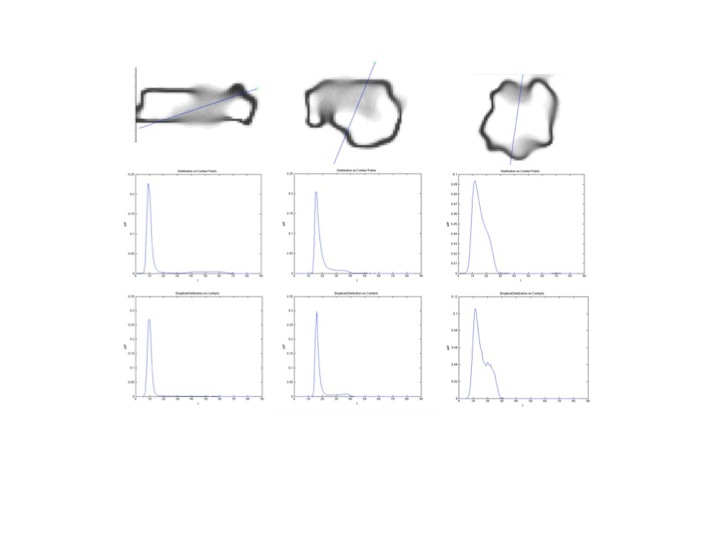
\includegraphics[scale = 0.3]{figures/Slide07.jpg}
\caption{Top: A surface with GPIS construction and line of action with the start pointed denoted by green x.
Middle: Theoretical distribution computed on contact point
Bottom: Empirically sampled distribution}
\vspace*{-10pt}
\label{fig:Contact_Dist}
\end{figure}

\begin{figure}[ht!]
\centering
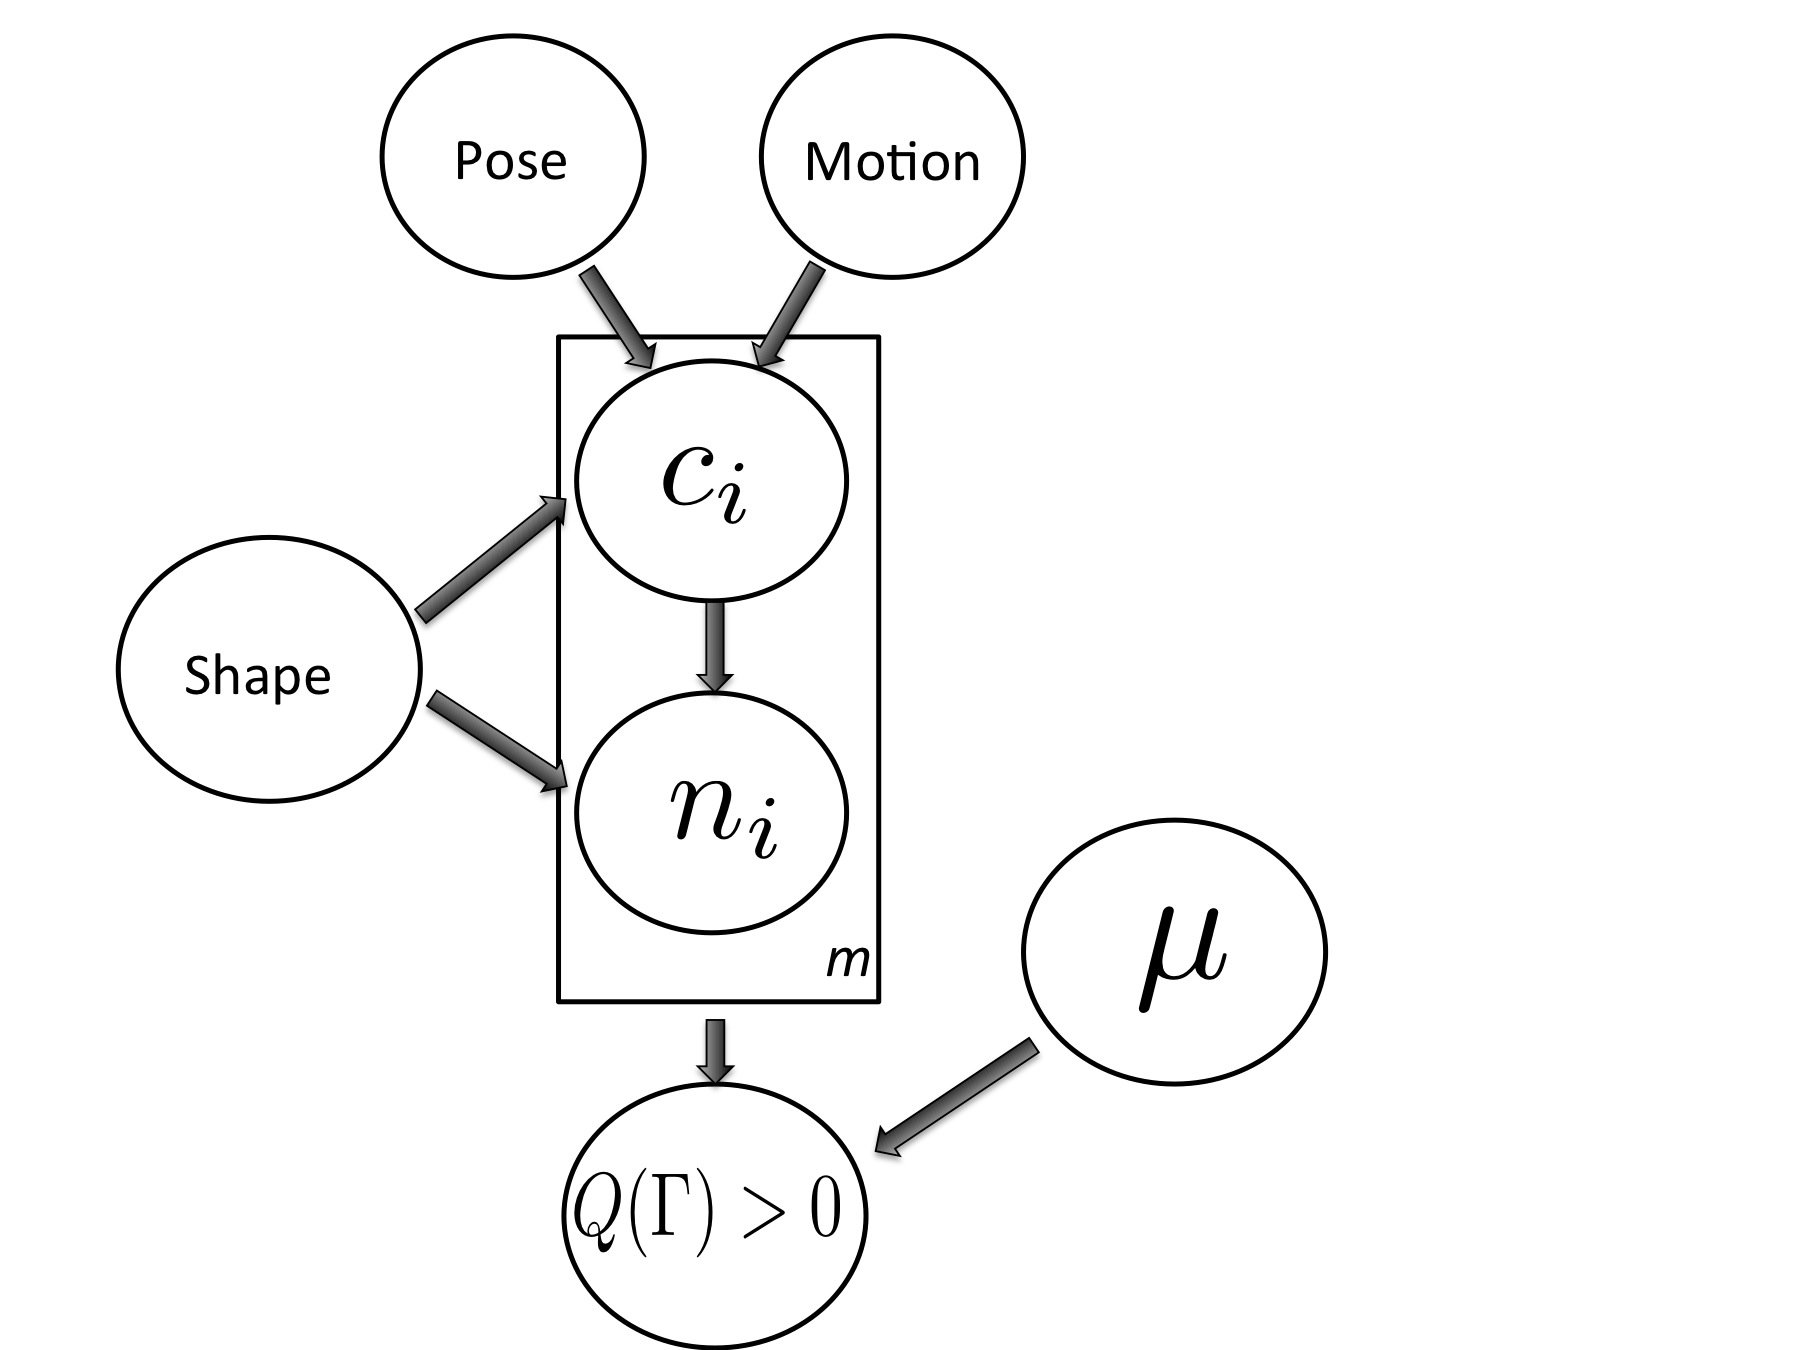
\includegraphics[scale = 0.3]{figures/Slide08.jpg}
\caption{Top: A surface with GPIS construction and line of action with the start pointed denoted by green x.
Middle: Theoretical distribution computed for surface normals
Bottom: Empirically sampled distribution}
\vspace*{-10pt}
\label{fig:Normal_Dist}
\end{figure}

To better understand the quality of grasp that our proposed metric will find, we present results on a variety of grasps as shown in Fig. \ref{fig:Grasps}. The numerical values in terms are presented in Table 2. 


\begin{figure}[ht!]
\centering
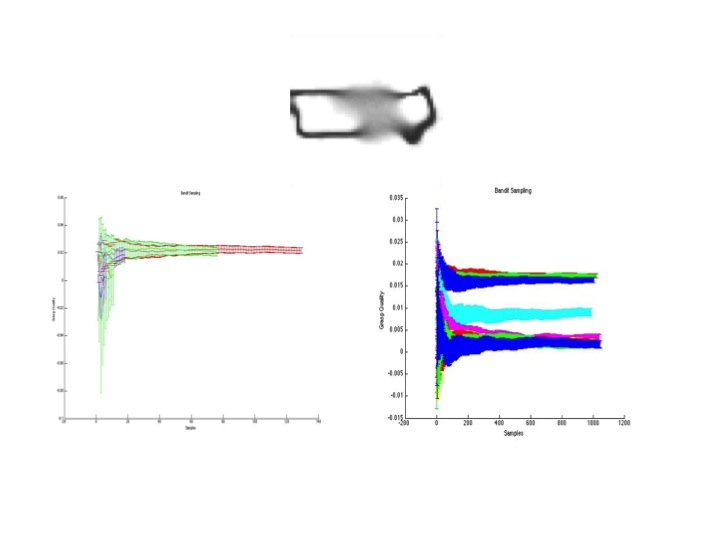
\includegraphics[scale = 0.3]{figures/Slide09.jpg} 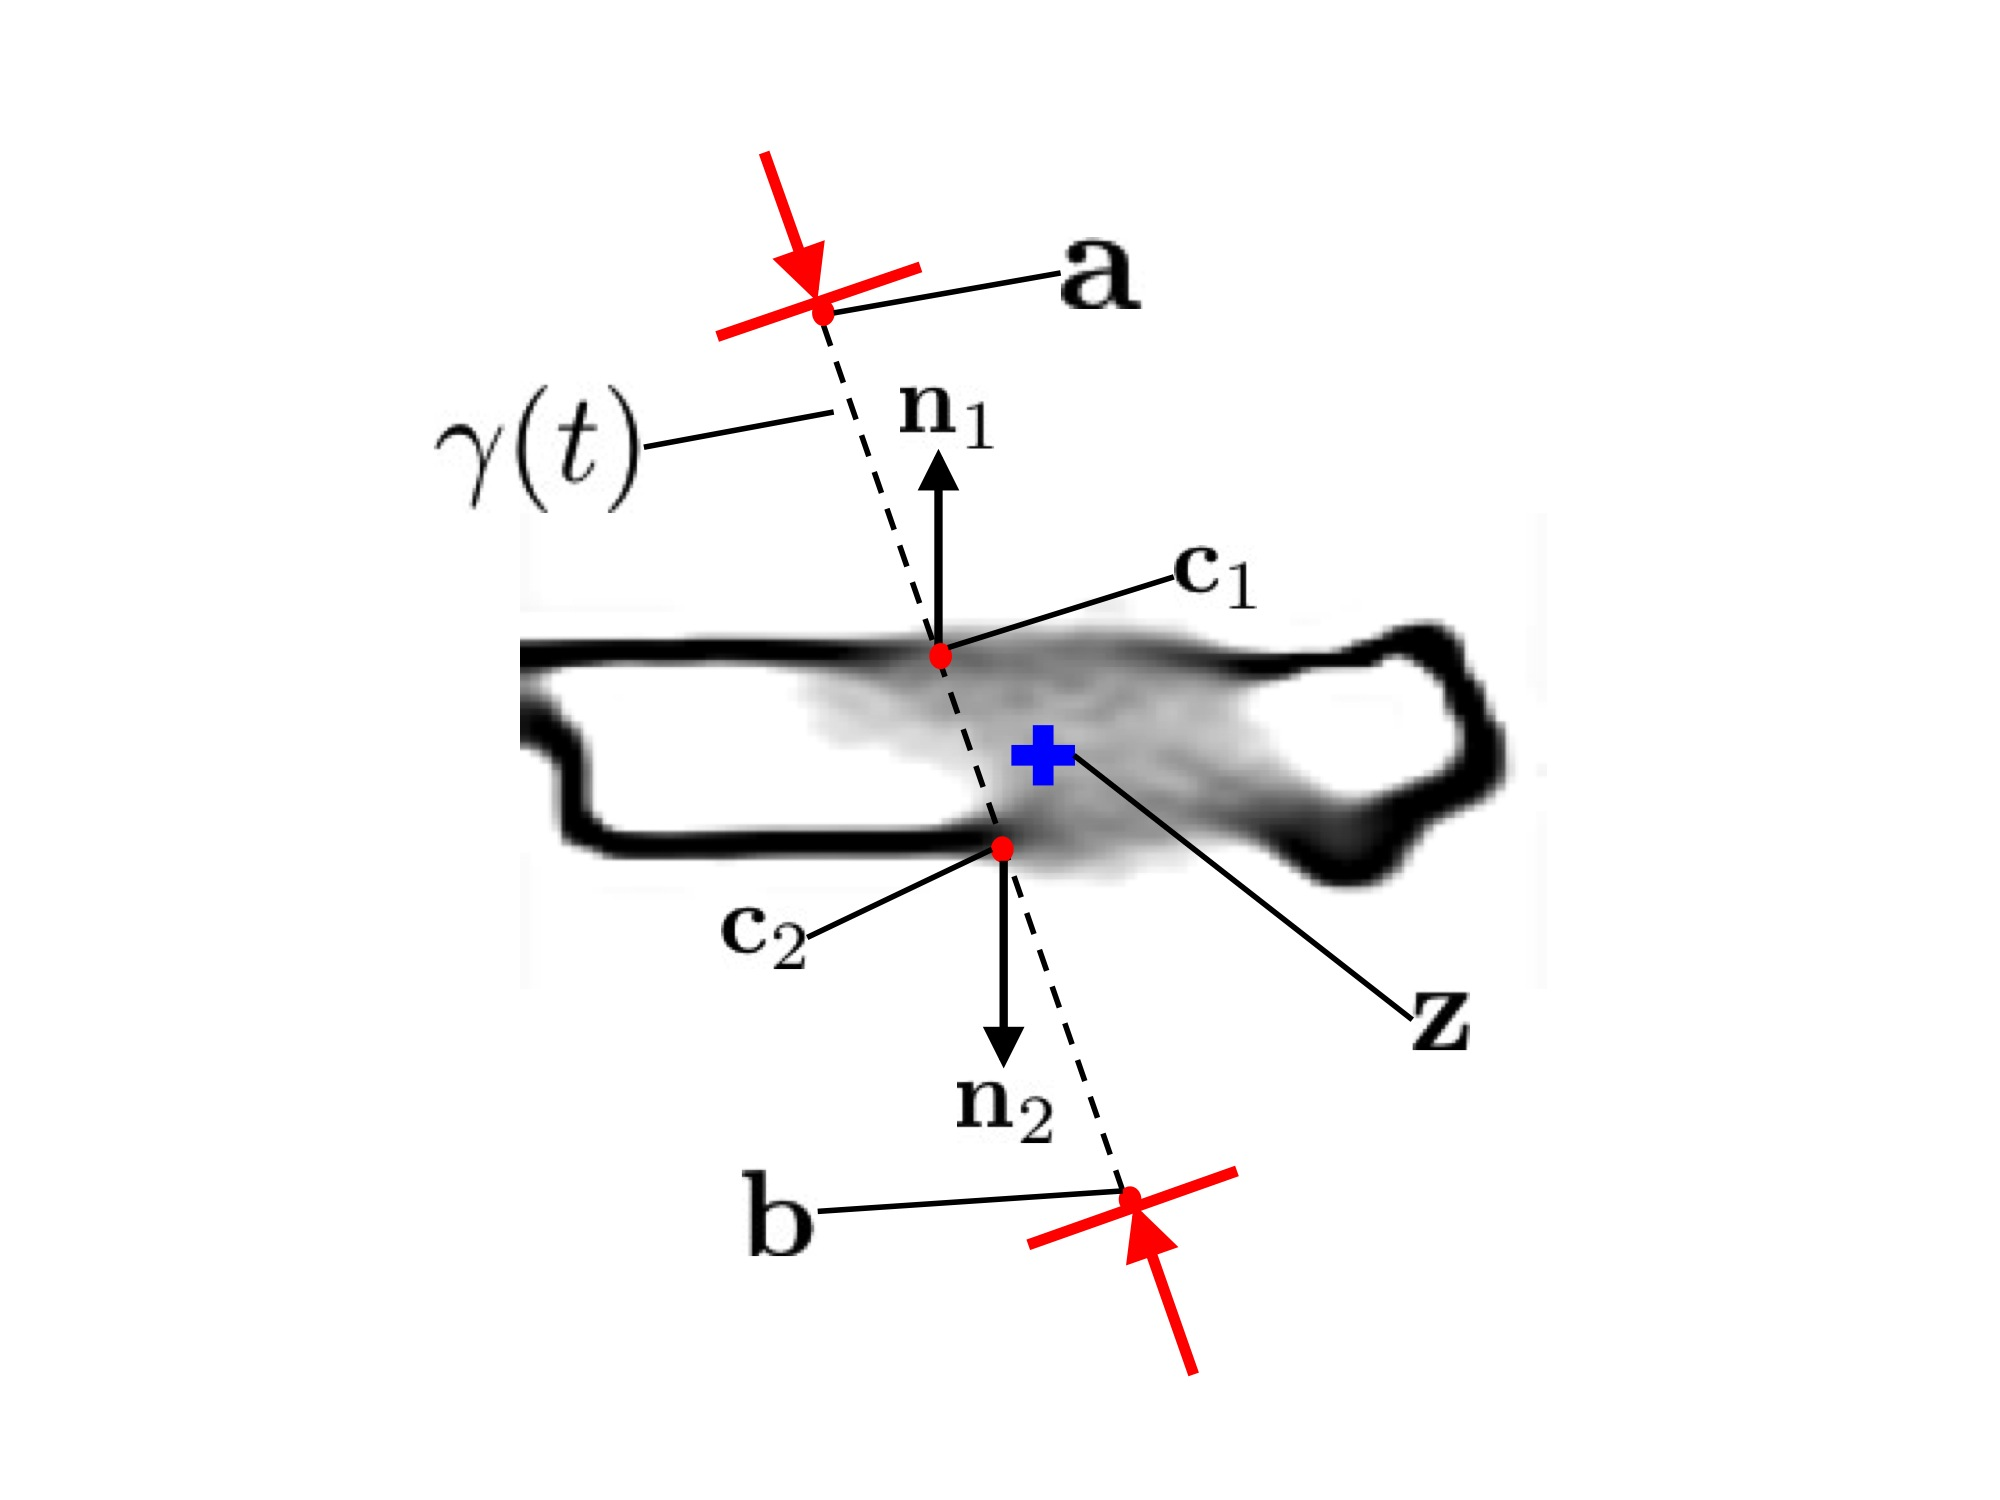
\includegraphics[scale = 0.3]{figures/Slide10.jpg}
\caption{Example grasps on the provided dataset with the histrograms of grasp quality given the uncertainity}
\vspace*{-10pt}
\label{fig:Grasps}
\end{figure}



\begin{table}[ht!]
        \begin{tabular}{ l | c c c c}
         Distribution & \bf Marker & \bf Tape & \bf Loofa & \bf Stapler \\ 
        \hline \\
         $\bar{Q(g)}$ & -0.003 & 0.022 & 0.000 &  0.018\\
        \hline \\
        var $Q(g)$ & 0.025 & 0.016 & 0.017 &  0.054\\
        \hline 
        $Q(\bar{g})$ & 0.030 & 0.024 & -0.012 & 0.014\\
        \hline 
        $b$ & 1.634 & 0.540 & 2.220 & 2.600 \\
        \hline 
        $h$ & 0.025 & 0.016 & 0.017 & 0.097 \\
        \hline 
        \end{tabular}
        \caption{A comparison of all the different values that characterize a grasp.}
		
\vspace*{-20pt}
\end{table}

\bibliographystyle{ieeetr}
\bibliography{references}

\end{document}
